

\documentclass{article}
\usepackage[utf8]{inputenc}
\usepackage{authblk}
\usepackage{setspace}
\usepackage{natbib}
\usepackage{hyperref}
%\usepackage{cite}
\usepackage[margin=1in]{geometry}
\usepackage{array}
\usepackage{graphicx}
\usepackage{caption}
\graphicspath{ {./figures/} }
\usepackage{subcaption}
\usepackage{amsmath}
\usepackage{lineno}
\usepackage{soul}
\usepackage{xcolor}
\sethlcolor{yellow}
\linenumbers

%%%%%%%%%%%%%%%%%
\title{Thesis outline}
\date{\today}
\author{Christophe Rouleau-Desrochers}
\begin{document}
%%%%%%%%%%%%%%%%%%%%%%%%%%%%%%

\maketitle


%<><><><><><><><><><><><><><><><><><><><>
% Introduction
%<><><><><><><><><><><><><><><><><><><><>
\section{Introduction}

% ============================
% 1. CC  X Phenology
% ============================
\subsection{Climate change impacts on tree phenology} 
Climate change impacts on biological systems and how phenological trends are already shifting with warming temperatures.\\
\textbf{1.1.1. Trends of spring and autumn phenological events and their drivers \citep{walther_ecological_2002} } \\
	1.1.1.1. changes in phenology \\ 
	1.1.1.2. Drivers of spring phenology (including forcing and chilling from paragraph of declining sensitivity) \\
	1.1.1.3. Drivers of autumn phenology \\ 
\textbf{1.1.2. How these shifts translate into effects on trees/forests not totally clear -- Pros and cons of early/late start of season:} \\  
\textbf{1.1.3.Growing season shifts consequences on forest ecosystems and services }


% ============================
% 1.2. NATURE OF THE PROBLEM
% ============================
\subsection{Nature of the problem and to address it} 

\textbf{1.2.1. Past phenological trends can help (or not) predict future phenological changes} \\ 
\textbf{1.2.2. The assumption that longer seasons lead to increased growth is called into question} \\ 
\textit{1.2.2.1. Absence of growth despite better conditions and strategies that can be used}  \\
\textit{1.2.2.2. Experiments} \\ 
\textit{1.2.2.3. Ground based observations} \\
\textbf{1.2.3. Goals of my thesis}\\
\subsection{Complexity of measuring growth} 
\textbf{1.3.1. Definition of growing season and growth} \\ 
\textbf{1.3.2. Traditional diameter measurements miss the resolution of the annual growth increment.} \\ 
\textbf{1.3.3. Dendroecology to analyses growth responses to changing growing season length}
\textbf{1.3.4. Primary and secondary growth do not start and end at the same time} * remove?


% ============================
% Research questions
% ============================
\subsection {Research questions} %emwJuly1 -- I think 'Tree Rings stuff' should move down and you should replace it with a paragraph on the complexity of measuring growth (and then make sure the sentence before it about your broad thesis goals focuses on growth) and maybe measuring growth with changing growing seasons! This would lead nicely into your research questions 
\begin {enumerate}
	\item \textbf{Fuelinex}: How do extended growing seasons affect tree growth across different species, both immediately (in the same year as the extended season) and in subsequent years?
	\item \textbf {CookieSpotters}: How phenological traits regulate tree growth in urban ecosystems?
\end {enumerate}

% ============================
% Hypothesis
% ============================
\subsection{Hypothesis}
\begin {enumerate}
	\item \textbf{Fuelinex}: Growing season extension modifies a tree’s capacity to sequestrate carbon and nitrogen, and this could lead to increased growth in the following season.
	\item \textbf{Fuelinex}: Species capable of accumulating nutrients after growth cessation while going through leaf senescence might exhibit growth increment in the following growing season
	\item \textbf{CookieSpotters}: The magnitude of the growth response to longer seasons will differ between juvenile and mature trees.
\end {enumerate}

% ============================
% Objectives and outreach
% ============================
\subsection{Objectives and outreach}
\begin {enumerate}
	\item \textbf{Fuelinex}: Assess tree species’ potential to prolong or stretch their activity schedule.
	\item \textbf{Fuelinex}:  Determine whether trees can absorb nutrients beyond their theoretical growing season.
	\item \textbf{Fuelinex}:  Examine if increased carbon pools translate into greater growth increment in the following growing season. 
	\item \textbf{CookieSpotters}: Investigate how the timing of phenological events affects growth across years for juvenile and mature trees
\end {enumerate}

%<><><><><><><><><><><><><><><><><><><><>
% Methods
%<><><><><><><><><><><><><><><><><><><><>
\section{Methods}

% ============================
% Fuelinex
% ============================
\subsection{Fuelinex}
\begin {enumerate}
	\item Full factorial design (Fig. 1)
%%%
\begin{figure}[p] 
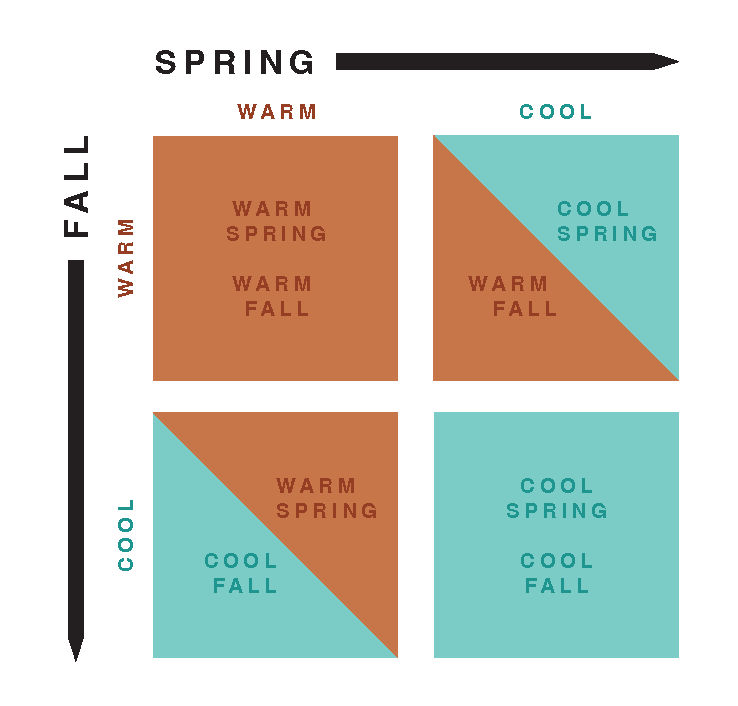
\includegraphics[width=1.1\textwidth]{FullFactorialFigure.pdf} 
\caption{Full factorial design of Cool/Warm Spring and Cool/Warm Fall}
\label{fig:sample}
\end{figure}
%%%
	\item 2-year experiment over 2024-2025 (Fig. 2 and 3)
%%%
\begin{figure}[p]
\includegraphics[width=1.1\textwidth]{Fuelinex_Design2024.pdf}
\caption{Experimental design of the different treatments that were performed during the growing season of 2024. The timeline displays the periods of the different measurements. Nutrient addition treatments are displayed by the black elipses}
\label{fig:sample}
\end{figure}
%%%
\begin{figure}[p]
\includegraphics[width=1.1\textwidth]{Fuelinex_Design2025.pdf}
\caption{Timeline displaying the periods of the different measurements during the growing season of 2025}
\label{fig:sample}
\end{figure}
%%%
	\item Nutrient addition
	\item Data: phenology, shoot elongation, diameter, height, biomass, tree rings
	\item Analysis: TBD
	\item Studied species (Table 1)

\end {enumerate}

%%%
\begin{table}[p]
\centering
\caption{Fuelinex species grouped by tree type, life history, and wood anatomy.}
\begin{tabular}{|>{\raggedright\arraybackslash}p{7cm}|p{5cm}|p{3cm}|p{1cm}|}
\hline
\multicolumn{4}{|c|}{\textbf{Deciduous Trees}} \\
\hline
\textbf{Common Name (Latin)} & \textbf{Life History Strategy} & \textbf{Wood Anatomy} & \textbf{n (approx)} \\
\hline
Bur oak (\textit{Quercus macrocarpa}) & Slow-growth, long life & Ring-porous & 87\\
Bitter cherry (\textit{Prunus virginiana}) & Fast-growth, short life & Diffuse-porous & 78\\
Box elder (\textit{Acer negundo}) & Fast-growth, short life  & Diffuse-porous & 90\\
Balsam poplar (\textit{Populus balsamifera}) & Fast-growth, short life  & Diffuse-porous &84 \\
Paper birch (\textit{Betula papyrifera}) & Fast-growth, short life  & Diffuse-porous &90\\
\hline
\multicolumn{4}{|c|}{\textbf{Evergreen Trees}} \\
\hline
White pine (\textit{Pinus strobus}) & Slow-growth, long life & & 89\\
Giant Sequoia (\textit{Sequoiadendron giganteum}) & Slow-growth, long life & & 54\\
\hline
\end{tabular}
\end{table}
%%%
% ============================
% Wildchrokie
% ============================
\subsection{Wildchrokie}
\begin {enumerate}
	\item Common garden from 2015 to 2023
	\item Four species within the Betulacea family (Table 2)
%%%
\begin{table}[p]
\centering
\caption{Wilchrokie species grouped by tree type, life history, and wood anatomy.}
\begin{tabular}{|>{\raggedright\arraybackslash}p{7cm}|p{5cm}|p{3cm}|p{1cm}|}
\hline
\multicolumn{4}{|c|}{\textbf{Deciduous Trees}} \\
\hline
\textbf{Common Name (Latin)} & \textbf{Life History Strategy} & \textbf{Wood Anatomy} & \textbf{n} \\
\hline
Paper birch (\textit{Betula papyrifera}) & Fast-growth, short life  & Diffuse-porous & 8\\
Yellow birch (\textit{Betula alleghaniensis}) & Moderate-growth, moderate life & Diffuse-porous & 21\\
Grey birch (\textit{Betula populifolia}) & Fast-growth, short life & Diffuse-porous & 29\\
Grey alder (\textit{Alnus incana}) & Fast-growth, short life & Diffuse-porous & 31\\
\hline
\end{tabular}
\end{table}
%%%
	\item Data: phenology, height, tree rings
	\item Analysis: Hierarchical model to understand how tree ring width relates to GDD
\end {enumerate}

% ============================
% Treespotters
% ============================
\subsection{Treespotters}
\begin {enumerate}
	\item Citizen scie nce project from 2015 to today (Table 3)
\begin{table}[h]
\centering
\caption{Treespotters species grouped by tree type, life history, and wood anatomy.}
\begin{tabular}{|>{\raggedright\arraybackslash}p{7cm}|p{5cm}|p{3cm}|p{1cm}|}
\hline
\multicolumn{4}{|c|}{\textbf{Deciduous Trees}} \\
\hline
\textbf{Common Name (Latin)} & \textbf{Life History Strategy} & \textbf{Wood Anatomy} & \textbf{n} \\
\hline
American basswood (\textit{Tilia americana}) & Fast-growth, moderate life & Diffuse-porous & 5\\
Eastern cottonwood (\textit{Populus deltoides}) & Fast-growth, short life & Diffuse-porous & 4\\
Northern red oak (\textit{Quercus rubra}) & Moderate-growth, long life & Ring-porous & 4\\
White oak (\textit{Quercus alba}) & Slow-growth, long life & Ring-porous & 5\\
Pignut hickory (\textit{Carya glabra}) & Slow-growth, long life & Ring-porous & 4\\
Shagbark hickory (\textit{Carya ovata}) & Slow-growth, long life & Ring-porous & 4\\
River birch (\textit{Betula nigra}) & Fast-growth, short life & Diffuse-porous & 5\\
Yellow birch (\textit{Betula alleghaniensis}) & Moderate-growth, moderate life & Diffuse-porous & 4\\
Sugar maple (\textit{Acer saccharum}) & Slow-growth, long life & Diffuse-porous & 5\\
Red maple (\textit{Acer rubrum}) & Slow-growth, long life & Diffuse-porous & 4\\
Yellow buckeye (\textit{Aesculus flava}) & Moderate-growth, moderate life & Diffuse-porous & 5\\
\hline
\end{tabular}
\end{table}

	\item Tree coring
	\item Data: phenology, tree rings
	\item Analysis: Hierarchical model to understand how tree ring width relates to GDD	
\end {enumerate}

\section{Timeline} 
Fig. **
%%%
\begin{figure}[h]
\includegraphics[width=1.1\textwidth]{ganttChart.pdf}
\caption{Gant chart displaying the different milestones to be done over 2025 and 2026}
\label{fig:sample}
\end{figure}
%%%

\section {References}
\bibliography{Exported_Items.bib}
\bibliographystyle{nature} % set citation style 


% old text
%\section*{Chapter 2.1. Wildchrokie: Phenological observations coupling with tree-ring width measurements for a 6-year common garden experiment} While the assumption that a longer growing season leads to increased growth is an intuitive and common one, recent evidence shows that this may not be the case. 
%How phenological season length relates to growth. This is a major question in fundamental biology, but also critical to forecasts of climate change itself, since most carbon models assume that plants experiencing longer seasons will sequester more carbon, but recent studies have called this assumption into question.


% ============================
% 2. Tree-ring stuff 
% ============================
%\subsection{Tree rings measurements as a proxy for growth}
%Using tree ring data to investigate the relationship between phenology and growth

%\begin{enumerate}
% 1)
%	\item Triggers and mechanisms behind growth onset, duration and rate.
%Growth onset and duration vary because of inter-annual differences in weather, with cambium reactivation in spring being highly dependent on temperature. 
% 2)
%	\item How radial growth is influenced by extreme weather events and their timing. 
%Growh rate increased by temperature, depends on \textbf{when} it is warmer. 
% Include in main text: Long seasons at low temperature will produce fewer cell rows than at warmer temperature.
% 3) 
%	\item Which is more important? How fast does a tree grow, or how long does it grow for?
%how growth rate may have a more direct influence on tree growth than the growing season length. 
% 4)
%	\item Methods to measure tree growth and why using tree ring images may better capture tree growth response than traditional diameter and height measurements.
% Include in main text: Diameter and height measurements are widely used to assess yearly biomass increment. However, these measurements are punctual and are often the cumulative result of many climatic events and constraints that occur during a tree's lifespan
%\end{enumerate}



\end{document}
